
\subsection{Axial Shielding Factor Measurements}

In these measurements, a witness cylinder was used as a magnetic
shield.  Small changes in the axial shielding factor are interpreted
as a change in the effective $\mu$ of the material.  This technique is
quite different than the usual mutual inductance techniques used by
other groups.  Our hope was that this geometry would give us more
confidence that the properties we were measuring were indeed related
to magnetic shielding properties rather than inherent properties of
the material.

\subsubsection{Magnetic Field Generation}

In order to measure the magnetic shielding factor, the witness
cylinder was placed within a homogeneous AC magnetic field.  The field
was created within the magnetically shielded volume of the prototype
magnetic shielding system (described previously in
Section~\ref{sec:previousmeasurement} in order to provide a good
magnetic environment.  A short solenoid inside the shielding system
was used to produce the magnetic field.
%The radius and the half
%length of the solenoid is 17.44~cm while the radius and the half
%length of our innermost prototype passive shield is 18.44~cm.
The solenoid has 14 turns with 2.6~cm spacing between the wires.  The
solenoid was designed so that the field produced by the solenoid plus
innermost shield approximates that of an infinite solenoid.  The
magnetic field generated by the solenoid was typically 1~$\mu$T.  The
solenoid current was varied sinusoidally at typically 0.01 to 10~Hz.
%The $\mu$ dependence of the reaction factor for the solenoid is known
%to be considerably smaller than the $\mu$ dependence of the axial
%magnetic shielding factor of the witness cylinder.  Hence the
%temperature dependence of the amplitude of the field measured by the
%fluxgate can be ascribed to changes of the witness cylinder, rather
%than changes in the innermost magnetic shield.


% Need to explain ``local coil'' as well, right here, right now.
% or just below, when Fig. geometry is shown.

\subsubsection{Witness cylinder and fluxgate magnetometer}

The witness cylinder was placed into this magnetic field generation
system as shown schematically in Fig.~\ref{fig:geometry}.  The
cylinder was held in place by a wooden stand.



A Bartington fluxgate magnetometer Mag-03IEL70 (low noise) measured
the magnetic field at the center of the witness cylinder.  The
fluxgate is a ``flying lead'' model, meaning that each axis is
available on the end of a short electrical lead, separable from the
other axes.  One ``flying lead'' was placed in the center of the
witness cylinder, the axis of the fluxgate being aligned with that of
the witness cylinder.  The fluxgate was held in place rigidly by a
plastic mounting fixture, which was itself mounted to the witness
cylinder.
% leftovers after Jeff's editing, which might be useful...
% A plastic rod with 2.5~cm diameter used to hold the fluxgate
% flying lead. A hole with a diameter of 0.8~cm was drilled along the
% axis of the plastic rod to reach the middle.  One ``flying lead'' (or
% axis) was held at the hollow center of the holder by a plastic set
% screw. The plastic rod was then placed along the axis of symmetry of
% the witness cylinder and coupled to it by using two plastic end caps
% that threaded onto the plastic rod.  In all data acquisitions, only
% one fluxgate flying lead was used.


To increase the resolution of the measured signal from the fluxgate, a
Bartington Signal Conditioning Unit (SCU) with a low-pass filter set
to typically 10-100~Hz and a gain set to typically $>50$ was used.
The signal from the SCU was demodulated by an SRS830 lock-in amplifier
providing the in-phase and out-of-phase components of the signal.
(The sinusoidal output of the lock-in amplifier reference output
itself was normally used to drive the solenoid generating the magnetic
field.)  The time constant on the lock-in was typically set to 3
seconds with 12~dB filter.

\begin{figure}
\begin{center}
   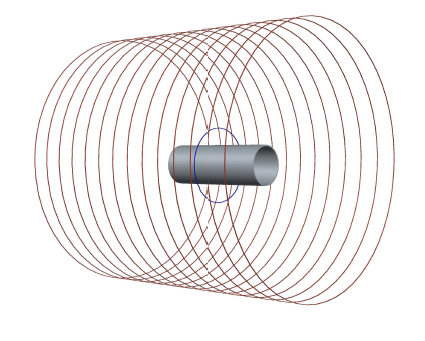
\includegraphics[width=0.8\textwidth]{geometry.PNG}
    \caption{Axial shielding factor measurement setup. The witness
      cylinder with a radius of 2.54~cm and a length of 15.2~cm is placed
      inside a solenoid with a radius and a half length of
      17.44~cm. The axis of symmetry is along the $z$-axis. The
      windings of the solenoid is shown in red. The blue coil with one
      turn is coupled to the witness cylinder and it has a radius of
      5~cm.  }
% Note to Jeff (self): fix this figure caption!!!
% (Need to look at it in the pdf form to think more about it.)
    \label{fig:geometry}
    \end{center}
\end{figure}

As shall be described in Section~\ref{sec:axialsyst}, a concern in the
measurement was changes in the field measured by the fluxgate that
could arise due from motion of the system components, or other
temperature dependences.  This could generate a false slope with
temperature that might incorrectly be interpreted as a change in the
magnetic properties of the witness cylinder.

To address possible motion of the witness cylinder with respect to the
field generation system, another coil was wound on a plastic holder
mounted rigidly to the witness cylinder.  The coil was one loop of
copper wire with a radius of 5~cm. The loop coil holder had inner
radius of 2.7~cm and an outer radius of about 5~cm.  Plastic set
screws in the holder fixed the loop coil to be coaxial with the
witness cylinder.

Systematic differences in the results from the two coils (the
solenoidal coil, and the loop coil) were used to search for motion
artifacts.  As well, some differences could arise due to the different
magnetic field produced by each coil, and so such measurements could
reveal a dependence on the profile of the applied magnetic field.  In
the end, no conclusive difference in the results from either coil
could be found.  This is described further in
Section~\ref{sec:axialsyst}.


\subsubsection{Temperature measurement and data acquisition}


%%%%%%%%%%%%%%%%%%%%%%%%%%%%%%%%%%%%%%%%%%%%%%%%%%%%%%%%%%
% It has been moved up from the systematic error section
%%%%%%%%%%%%%%%%%%%%%%%%%%%%%%%%%%%%%%%%%%%%%%%%%%%%%%%%%%
%
%The mu-metal alloy has a thermal conductivity of 0.35
%W/(cm$\cdot$K). Therefore, four thermocouples placed on different
%spots on the witness cylinder to correct for small temperature
%differences on each end of the witness cylinder.  In these
%measurements, the farther side of the passive shields had the end caps
%while the other side was left open to give access to the interior
%region. Based on the magnetic field maps inside the passive shields,
%for 10 $\mu$T applied magnetic field, the stability of the field was
%to 0.1 $\mu$T level and the magnetic field was even more stable closer
%to the closed side of the passive shields. Therefore the witness
%cylinder was pushed to the side with the end caps on the passive
%shields.


The temperature of the witness cylinder was measured by attaching four
thermocouples at different points along the outside of the cylinder.
To reduce any potential magnetic contamination, T-type thermocouples
were used, which have copper and constantan conductors.  (K-type
thermocouples are magnetic.)  Two thermocouples were attached to the
edges of the witness cylinder and the other two were attached on
opposite sides in the middle.  This allowed us to observe the
temperature gradient along the witness cylinder.

Thermocouple readings were recorded by a National Instruments NI-9211
temperature input module.  The magnetic field (signified by the
lock-in amplifier readout) and the temperature were recorded at a rate
of 0.2~Hz.

Temperature variations in the experiment were driven by ambient
temperature changes in the room, although forced air and other
techiques were also tested.  These are described further in
Section~\ref{sec:axialsyst}.


\subsubsection{Data and Interpretation}

An example of the typical data acquired is shown in
Fig.~\ref{fig:B_vs_Temp}.  The field amplitude produced by the
solenoid was 2.6~$\mu$T, at a frequency of 1~Hz.
Fig.~\ref{fig:B_vs_Temp}(a) shows the temperature of the witness
cylinder over a four-day measurement.  The temperature changes are
about 3.5~K and are caused by temperature variations of the
laboratory.
% The following statement belongs more in the systematic errors section:
%
% For $f\lesssim 1$~Hz most of the measured fluxgate signal is in the
% in-phase component.
%
The magnetic field $B$ is anti-correlated with the temperature trend
in an shown in Fig.~\ref{fig:B_vs_Temp}(b).  Here, $B$ is the sum, in
quadrature, of the amplitudes of the in-phase and out-of-phase
components.  Magnetic field is then interpreted to depend on the
temperature, and they are graphed as a function of one another in
Fig.~\ref{fig:B_vs_Temp}(c).  The slope of Fig.~\ref{fig:B_vs_Temp}(c)
has been calculated using a linear fit to the data.  In this
measurement, the slope is found to be
$\frac{1}{|B|}\frac{d|B|}{dT}\simeq -1.5\%$/K.

Deviations from the linear straight-line dependence can be seen in the
data.  For example at the start of the data-taking, the slope is
almost zero.  This is typical of the data that we acquired, that the
magnetic field as a function of temperature would not necessarily lie
along a straight line, but rather would have different slope
temporarily after changing the sign of the temperature slope with
time.

Another feature of the data was that, on subsequent similar
measurements, the value of the slope would not be the same, on a
measurement-to-measurement basis.

A comprehensive set of systematic studies of the factors affecting the
slope were performed, and these are presented in
Section~\ref{sec:axialsyst}.  A basic summary of those studies was
that no external parameter was found that could explain the periodic
changes in slope that were observed.  Based on these studies, we
expect the change in slope is either due to an irreproducibility in
the magnetic properties of the material, or due to an uncharacterized
systematic error such as a long-time mechanical relaxation of some
element of the apparatus.

To express this inherent uncertainty in the slope, we phrase our
result as a range of slopes that were typical of data acquired over
time periods of $\sim$ days.  In general, we measured
0.3\%/K~$<\vert\frac{1}{B}\frac{dB}{dT}\vert<$~2.3\%/K with the sign
% Jeff got to here on pass 2.
% question for Taraneh: should be solenoidal coil only? or what's the
% answer for solenoidal coils as compared to loop coil?  answer from
% Jeff and Taraneh, so far: this needs to be fixed.  We should put
% both measurements up here and explain the difference.
being negative.  The range also encompasses the typical deviation from
a linear $B(T)$ in the data (for example, those seen in
Fig.~\ref{fig:B_vs_Temp}(c).).  Since the data cannot be embodied by a
single temperature slope, the experiment tends to set a scale and sign
for the possible temperature dependence, rather than a value.

\begin{figure}
\begin{center}
   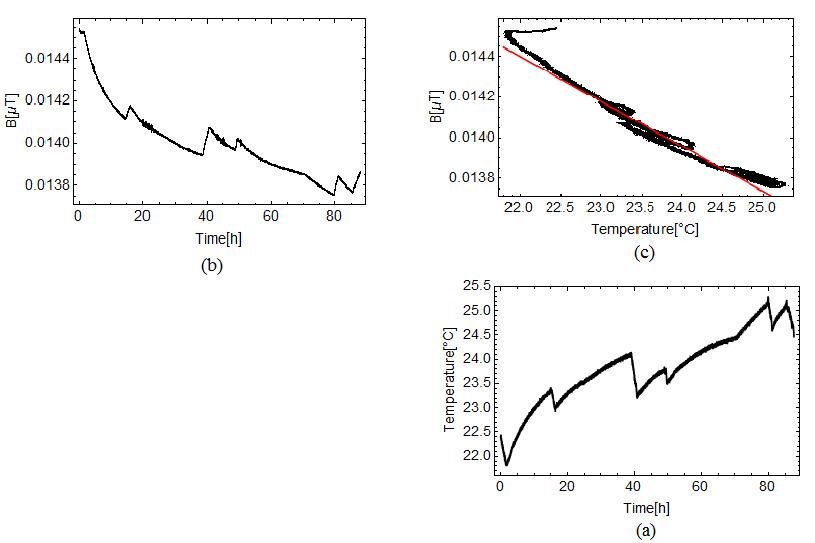
\includegraphics[width=0.5\textwidth]{B_vs_T.png}
% Taraneh to do: vertical label should likely be ``B amplitude'' or
% ``amplitude of measured field'', to make it clear that this has been
% multiplied by sqrt(2).  Either that, or the sqrt(2) should be
% removed to avoid inconsistency with the transformer measurements
% presented later.
    \caption{Ambient temperature and shielded magnetic field
      amplitude, measured over a 90 hour period. (a) temperature of
      the witness cylinder as a function of time.  (b) magnetic field
      amplitude measured by fluxgate at center of witness cylinder
      versus time.  (c) magnetic field versus temperature. The red
      line in (c) is a linear fit to data. At 22$^\circ$C,
      $\frac{1}{|B|}\frac{d|B|}{dT}=-1.5\%$/K.}
% This was actually measured by the local coil!!!
% This was actually measured by the local coil!!!
    \label{fig:B_vs_Temp}
    \end{center}
\end{figure} 

% This was actually measured by the local coil!!!
% This was actually measured by the local coil!!!

% Taraneh says: Several data from March 2015 is now added to the long
% report on Plone. We might need to consider replacing this graph with
% another one. I am aware of the fact that the graphs in the long
% report are not publication quality. But once we decide on some
% particular data, I will make nicer looking graphs.

\subsubsection{Systematic Studies\label{sec:axialsyst}}

\paragraph{Methods of Temperature Variation}

In addition to ambient temperature changes, we tried other methods of
forced temperature change.  In one design, Tygon tubing was wrapped
around the witness cylinder in a spiral pattern to flow water whose
temperature could be controlled.  Mechanical stability issues clearly
dominated the systematic uncertainty in that measurement.  When water
was flowing, the flexibility of the tubing caused a movement in the
witness cylinder.  The motion was itself temperature-dependent because
warmer water caused the tubing to become more supple.  To address this
effect, the tubes were replaced by copper tubing.  But in this case,
the challenge was to create enough contact between the tubes and the
witness cylinder which was not successful. In another design, a TEC
was replaced with the tubing. The main issue with this design was that
it did not provide enough cooling for the witness cylinder and also it
was creating only local temperature changes on the witness
cylinder. In addition, despite of using heat sinks, the heat created
by the TEC itself made it very inefficient.  We also tried using
forced air to heat the witness cylinder.  This worked rather well, but
the heating had to be done slowly in order to avoid temperature
gradients across the apparatus, including the witness cylinder.  In
the end, using the ambient temperature changes in the room gave the
most reproducible results.  These followed a relatively stable diurnal
cycle with the function of the building's air conditioning system.

Although for most of the measurements the general trend of $B(T)$
graphs was consistent, the shape and positions of the nonlinear parts
of $B-T$ graphs were changing.  The changes in the $B$ vs.~temperature
slope always correlate with sharper changes in the temperature with
time.  The effect is most pronounced when a temperature that is
decreasing with time suddenly changes to increasing, or vice-versa.
However, we have incorporated the uncertainty from this effect into
our stated range of values.




%\paragraph{Final Design} 

% This has all been said and could be deleted, I think:

%final design
%The final design included the witness cylinder, which was placed with
%a holder inside the innermost prototype passive shield. The
%temperature variations of the witness cylinder was due to the
%temperature changes in the room which was following the on and off
%cycles of the building air conditioner.
%A Bartington magnetic field
%sensor (fluxgate) was hold inside the witness cylinder at the centre
%by plastic holder. The signal from the sensor was then demodulated by
%an SRS830 lock-in amplifier. To convert the final measured voltage
%from the sensor to $\mu$T, the sum in quadratures of the in-phase and
%out of phase components of the lock-in amplifier was multiplied by the
%scaling factor on the magnetic field sensor which is 7 $\mu$T/V.


%%%%%%%%%%%%%%%%%%%%%%%%%%%%%%%%%%%%%%%%%%%%%%%%%%%%%%%%%%%%%%%%%%%%%%
% This is all new and needs to move up to the apparatus section: (done)
%%%%%%%%%%%%%%%%%%%%%%%%%%%%%%%%%%%%%%%%%%%%%%%%%%%%%%%%%%%%%%%%%%%%%%
% The
% mu-metal alloy has a thermal conductivity of 0.35
% W/(cm$\cdot$K). Therefore, four thermocouples placed on different
% spots on the witness cylinder to correct for small temperature
% differences on each end of the witness cylinder.  In these
% measurements, the farther side of the passive shields had the end caps
% while the other side was left open to give access to the interior
% region. Based on the magnetic field maps inside the passive shields,
% for 10 $\mu$T applied magnetic field, the stability of the field was
% to 0.1 $\mu$T level and the magnetic field was even more stable closer
% to the closed side of the passive shields. Therefore the witness
% cylinder was pushed to the side with the end caps on the passive
% shields.
%%%%%%%%%%%%%%%%%%%%%%%%%%%%%%%%%%%%%%%%%%%%%%%%%%%%%%%%%%%%%%%%%%%%%%

% Another list
% - amplitude measurement on oscilloscope (no lock-in). (done)
% - speed of temperature change? temperature homogeneity?  (not here yet) 
% - other methods of cooling and why they didn't work. (not here yet)(done)
% - magnetic contamination by thermocouples (done)

% The above list maybe explains other possible variations on the
% method that you tried that all seemed to have worse systematic
% errors.

% Then, a list of systematic errors once you settled on the final
% measurement technique...

% - field profile/homogeneity (done)
% - mechanical stability (done)
% - thermal expansion (done)
% - temperature dependence of fluxgate and SCU (done)
% - temperature dependence of lock-in (done)
% - temperature dependence of coil resistance (not here yet) (done)
%    - Cupron/etc. study. plus
%    - measuring across the precision resistor
% - null measurement (Cu, and why it doesn't give the whole story, not here yet) (done)
% - effect of endcaps? (influence of external fields, not here yet)(done)
% - temperature dependence of reaction factor (negligible, not here yet)(done)
% - degaussing (not here yet)(done)
% - measurements on different witness cylinders? (not here yet)(done)
% - vibrations of the building?(done)
% - ...
%
% Another list is on the oldelog somewhere.  Please find it.
% The above list is longer and inclusive of the old list.
% See oldelog entry 141 in Magnetic Fields.
%
% This list of systematics is addressed now...

\paragraph{Field profile dependence and mechanical stability}

As mentioned earlier, a concern in the measurement was that motion of
the witness cylinder, the solenoidal coil, and the innermost magnetic
shield relative to one another could generate a false temperature
slope.  Another concern was that the spatial variation of the magnetic
field generated by the coil could somehow affect the measurement.  To
address these concerns, a loop coil rigidly mounted to the witness
cylinder was used to search for any differences compared to results
measured with the solenoidal coil.

The result of this study was that it did not reduce the typical slopes
measured, nor improve their reproducibility.  In the end, repeated
measurements of temperature slopes using the loop coil fell in the
range
0.4\%/K~$<\vert\frac{1}{B}\frac{dB}{dT}\vert<$~1.5\%/K.
% 0.5 is from Page 15 of Taraneh's summary.
% 0.4 is seen on Page 34 of Taraneh's logbook, Volume 1, Aug 2014-Dec 2015.
% 1.5 is from the Figure showed in the paper (page 14 of Taraneh's summary).
Similar measurements for the solenoidal coil yielded
0.3\%/K~$<\vert\frac{1}{B}\frac{dB}{dT}\vert<$~0.8\%/K.
% 0.3 is from Page 30 of Taraneh's summary
% 0.75 is from Page 34 of Taraneh's logbook, Volume 1, Aug 2014-Dec 2015.

% Jeff notes: these results should be stated as the primary results,
% right after/near the figure of the data.

% Taraneh to do: make a comment on H, right here, right now.  We
% should have a value for both the solenoidal coil and the loop coil.
% You might have to force Jeff to get it from his FEMM simulations.

In general, the slopes measured with the loop coil are larger than for
the solenoidal coil.  A partial explanation of this difference is
offered by the field profile generated by each coil, and its
interaction with the witness cylinder.  This is addressed further in
Section~\ref{sec:axialsims}.

However, the range of slopes measured in different trials still varied
within the stated ranges.  We conclude that whatever is causing the
slopes to change periodically is likely unrelated to motion of the
witness cylinder relative to the magnetic elements in the system.


% What is the value of the systematic error deduced from this study?
% I would say that the result of this study was that we got similar
% data to Fig. 3(c).  Therefore the systematic error due to field
% profile is smaller than the unknown systematic error of Fig. 3(c)
% and similar figures.  also partly addresses possible changes in
% reaction factor with temperature. (done)

Other potential motion artifacts due to thermal expansion of
components was also considered.  The thermal expansion coefficient of
mu-metal is $\sim$10~ppm/K~\cite{kruppvdm}.  However if the witness
cylinder expands uniformly in both thickness and radius, the shielding
factor is to first order unchanged.  In general, even unnatural
asymmetric and twisting motions of the fluxgate sensor and witness
cylinder tended to generate temperature slopes in the magnetic field
at the level $<30$~ppm/K.  The general homogeneity of the magnetic
field at the fluxgate sensor position and of the applied magnetic
field within which the witness cylinder was placed aided in minimizing
motion artifacts.

% http://nuclear.uwinnipeg.ca/oldelog/Magnetic+Fields/141
%As another mechanical stability study, the movement of the Bartington
%fluxgate flying lead due to thermal expansion was estimated. If the
%fluxgate flying lead move about 1 mm normal to its axis of symmetry
%which is parallel to the axis of the witness cylinder, the magnetic
%field will change about 30~ppm/K over 20~K temperature changes.

% %vibration
% Since the experiment site is located at the heart of downtown it is
% also possible that vibrations of the building affected the experiment
%setup and its machanical stability.
% Jeff says:  I can't think of much to say here.


%effect of the end caps

% Taraneh's version:

% In this experiment, one side of our prototype passive shield was
% closed with the end caps while the other side left open for easier
% access to the interior region. The result of the magnetic field map
% inside the prototype shield when the solenoid was turned on showed
% that closer to the far side of the shield, where the shield is closed,
% the magnetic field is more uniform. For a 10$\mu$T applied magnetic
% field the maximum change of the magnetic field along the axis of the
% passive shield was the order of 0.1~$\mu$T.  Therefore the witness
% cylinder was pushed to the far side of the prototype shield to reduce
% the non uniformity of the magnetic field.
% This is from oldElog entry 146: field map by Andrew Harrison

% Jeff's version (slightly shorter)

% As stated in Section~\ref{sec:axialapparatus}, the measurements were
% conducted within the magnetically shielded volume inside our
% prototype magnetic shields.  Most of the measurements were conducted
% with the endcaps of this shielding system removed on one side.  No
% systematic effect was found to arise from the removal of the
% endcaps.  The only effect was that the field produced by the
% solenoid was somewhat less homogeneous, which could easily be
% accounted for by moving the witness cylinder slightly closer to the
% side which has its endcaps on.  This was verified by measuring a
% magnetic field map of the region.

% Jeff's final version

% say nothing - this is an unimportant detail.  It had no effect on
% the measurement.  As far as we know, we would get the same value
% endcaps on or off.  I think it is more confusing to raise some
% possible issue about it and then say it wasn't a problem.

%temperature dependence of reaction factor
As the witness cylinder was put through its diurnal heating and
cooling cycles, so too was the magnetic shield within which the
apparatus was placed.  Since this magnetic shield is used as a flux
return, especially for the solenoidal coil, a concern could be that
the measurement confounds temperature dependence of the flux return
with the temperature dependence of the shielding factor of the
solenoid.  We want to clarify that this cannot be the case: any change
in $\mu$ of the flux return will have an exceedingly small effect on
the field produced by the solenoid.  This is perhaps best demonstrated
by Fig. \ref{fig:Magnetic_Field}, where the reaction factor in a
similar cylindrical geometry is graphed as a function of $\mu$.  Based
on our measurements, this limits systematic errors from such an effect
to be $<200$~ppm/K.

% This number above comes from:

% mu/B dB/dmu = 0.01

% times

% 1/mu dmu/dT < 2%/K

%degaussing
The magnetization of the witness cylinder changes the magnetic
permeability of the material and so the shielding factor changes.  Our
studies of degaussing the witness cylinder were consistent with
studies that we will report in
Section~\ref{sec:transformerdegaussing}.  Essentially, if the shields
were degaussed, or if they were left for long periods of time in the
small AC field generated by the solenoid, the results for temperature
dependences were similar.  Improper degaussing procedures were found
to induce long-term drifts in the measurement, uncorrelated with
temperature.  We do not include such data when quoting our
measurements of temperature slopes.  We do think that part of the
range of slopes that we measured is due to the magnetic properties of
the material, and that it is possible that some of this range is yet
due to insufficient degaussing on our part.  This is something we plan
to improve in planned future experiments on DC field stability.



\paragraph{Temperature slopes of various components of the apparatus}

The temperature coefficients of various components that could affect
the measurement were also considered.

The Mag-03IEL70 Bartington magnetic field sensor has a scaling
temperature coefficient of 15~ppm/K~\cite{bib:bartman}.  There is also
temperature coefficient for the offset of these sensors, but this is
irrelevant for this measurement because of the AC fields and
demodulation technique used.

The SRS830 lock-in amplifier has 50~ppm/K amplitude
stability~\cite{bib:lockin}.
% We did this for the transformer technique.
% Yes, but I think it is valid for this measurement as well, so let's put
% it here.
To further test this, the lock-in amplifier was connected to the coil
through a 1~$\Omega$ resistor with small temperature coefficient.  The
voltage across the resistor was measured with the lock-in amplifier
itself.  Any change would then be interpreted as a change in the
current supplied to the coil by the lock-in amplifier.  The measured
temperature dependence was always $<0.1$\%/K.

% To address this effect, another measurement conducted with local coil
% with Cupron wire windings. Cupron has higher resistivity compared to
% copper wires. The results showed no linear correlation between the
% measured magnetic field and the temperature of the witness cylinder.

% Taraneh asks:  The results?  Stride gum?  What to say?

% Jeff responds: I am not sure what to say about these results.  We
% didn't do the same measurement with the 1 Ohm resistor, I think, so
% it's hard to say if it was a problem with the temperature
% coefficient of resistance, or some geometrical change due to
% temperature change, or what.  Basically it is a confusing result in
% a somewhat weird experimental setup.

%Taraneh: I calculated from the long summary
The stability of the system was also tested by replacing the mu-metal
witness cylinder with a copper cylinder of very similar dimensions.
All other components of the system were the same.  The apparatus was
then run through its usual experimental cycle over several days.  For
all such measurements the temperature dependence of the demodulated
magnetic was $<0.1$\%/K.  This kind of measurement is unable to
address all possible systematic uncertainties.  For example, if moving
the mu-metal witness cylinder due to some thermal expansion would
change the field at the site of the fluxgate, moving the copper
cylinder will not make the same change.  Nonetheless it is an
encouraging result that the system does not measure a strong
temperature dependence of the magnetic field when no mu-metal witness
cylinder is present.  The magnitude of the magnetic field measured at
the fluxgate sensor was larger during these measurements because of
the lack of magnetic shielding from the copper.  So, in some tests the
magnetic field generated by the reference channel of the lock-in
amplifier was reduced to search for any problems arising from smaller
fluxgate signals.  No difference was seen within the upper bound
stated above.

\paragraph{Different Witness Cylinders}

The manufacturer of our prototype magnetic shields provided us with
three witness cylinders.  All three were used in these measurements.
Different cylinders possessed systematically different temperature
slopes, although always within the ranges quoted above.  These changes
are believed to arise from the manufacturing and annealing process.
It is known that the take-out temperature in the annealing process has
a strong effect on the temperature slopes measured at
50~Hz~\cite{bib:kruppdatasheet}.



% Two possibilities:

% 1. unknown systematic error(s)

% 2. complicated material properties that don't follow a straight line
% could depend on material history themselves.

% Therefore we state a range which should be indicative of the scale
% of possible temperature dependence.


\subsubsection{Geometry correction and determination of $\mu(T)$\label{sec:axialsims}}

To relate the data to $\mu(T)$, the shielding factor of the witness
cylinder as a function of $\mu$ must be known.  Finite element
simulations in FEMM and OPERA were performed to determine this factor.

Combining the measurement and the simulations, the temperature
dependence of the effective $\mu$ (at $\mu=20 000$, which is consistent
with our measurements) can be calculated by
\begin{equation}
\frac{1}{\mu}\frac{d\mu}{dT}=-\frac{\frac{1}{B}\frac{dB}{dT}}{\frac{\mu}{B}\frac{dB}{d\mu}}.
\end{equation}

From the simulations the ratio $\frac{\mu}{B} \frac{dB}{d\mu}$ was
calculated.  A linear model of the material was used where
$\bold{B}=\mu \bold{H}$ and $\mu$ is a constant independent of
$\bold{H}$.  The term $\frac{\mu}{B}\frac{dB}{d\mu}\neq 1$ because the
witness cylinders are open ended, and hence even for very large
$\mu\rightarrow\infty$ the shielding factor asymptotically approaches
a constant rather than infinity.

The simulations differed slightly in their results, dependent on
whether OPERA or FEMM was used, and whether the solenoidal coil or
loop coil were used.

Based on the simulations, the result is
$\frac{\mu}{B}\frac{dB}{d\mu}=0.42-0.50$ for the solenoidal coil, with
the lower value being given by FEMM and the upper value being given by
a 3D OPERA simulation, for identical geometries.  This is somewhat
lower than the value suggested by
Paperno~\cite{bib:paperno-open-ended} in his fits to simulations
performed in OPERA, which we estimate to be 0.6.  We adopt our value
since it is difficult to determine precisely from
Ref.~\cite{bib:paperno-open-ended}.  For the loop coil, we determine
$\frac{\mu}{B}\frac{dB}{d\mu}=0.56-0.65$, the range being given again
by a difference between FEMM and OPERA. These are presented in the second left column of Table~\ref{tab:axialsummary}. The third column from left summarizes the values of $B(T)$ measurements for both coil geometries discussed earlier in this section. The last column is the ratio of the third to the second column. 



\begin{table}
\begin{tabular}{|c|c|c|c|}
\hline 
  & $\vert \frac{\mu}{B}\frac{dB}{d\mu}\vert$ & $\vert \frac{1}{B} \frac{dB}{dT}\vert$~(\%/K) & $\frac{1}{\mu}\frac{d\mu}{dT}$~(\%/K) \\ 
\hline 
Solenoidal Coil & 0.42-0.50 & 0.3-0.8 & 0.6-1.9 \\ 
\hline 
Loop Coil & 0.56-0.65 & 0.4-1.5 & 0.6-2.7 \\ 
\hline 
\end{tabular} 
%\caption{A table to be filled in by Taraneh, and described in this
% caption and the surrounding text.}
\caption{The result of OPERA and FEMM simulations and the shielding factor measurement as well as the temperature dependence of $\mu$ for solenoidal and loop coil is summarized here. More detail is provided in the text.}
\label{tab:axialsummary}

\end{table}


Taking all these systematics into account, in this method it was found
that 0.6\%/K~$\lesssim\frac{1}{\mu}\frac{d\mu}{dT}\lesssim 2.7\%$/K.
This is quoted for a typical $H$ amplitude of XXX and a frequency of
1~Hz.

% Taraneh to do: look up number XXX for $H$.



%\begin{itemize}
%\item Describe experimental setup and important considerations
%  (e.g. relationship of data to effective $\mu$)
%\item Explain B, H, f, and dominant systematic effects.
%\item One figure of experimental setup?
%\item One data graph?
%\item State overall result and systematic error.
%\end{itemize}
